
\documentclass[12pt]{article} % Use A4 paper with a 12pt font size - different paper sizes will require manual recalculation of page margins and border positions

% Generated with LaTeXDraw 2.0.8
% Mon Jun 17 19:00:40 EDT 2013
\usepackage[usenames,dvipsnames]{pstricks}
\usepackage{epsfig}
\usepackage{pst-grad} % For gradients
\usepackage{pst-plot} % For axes
\usepackage[left=1.3cm,right=4.6cm,top=1.8cm,bottom=4.0cm,marginparwidth=3.4cm]{geometry} % Adjust page margins
\usepackage{amsmath} % Required for equation customization
\usepackage{amssymb} % Required to include mathematical symbols
\usepackage{xcolor} % Required to specify colors by name
\usepackage{amsthm}
\usepackage{float}
\usepackage{tikz}
\usetikzlibrary{shapes,backgrounds,trees}
\usepackage{wasysym}

\makeatletter
\newcommand{\mytag}[2]{%
  \text{#1}%
  \@bsphack
  \protected@write\@auxout{}%
         {\string\newlabel{#2}{{#1}{\thepage}}}%
  \@esphack
}
\makeatother

\setlength{\parindent}{0cm} % Remove paragraph indentation
\newcommand{\tab}{\hspace*{2em}} % Defines a new command for some horizontal space
%\newcommand{\choose}[2]{\left(\begin{matrix}
%{#1}\\{#2}
%\end{matrix}\right)}
\date{}
\title{Introduction to Probability Theory - Lecture 15}
%----------------------------------------------------------------------------------------

\newtheorem{defn}{Definition}
\newtheorem{example}{Example}
\newtheorem{prop}{Proposition}
\newtheorem{exer}{Exercises}
\newtheorem{thm}{Therorem}
\begin{document}
\maketitle

\section{Important Named Continuous Distributions - Continued}
\subsection{The Gamma Distribution - Continued}
Recall from last time, we defined the gamma function: 
\begin{defn}
The gamma function, denoted $\Gamma(\kappa)$ is defined to be:
$$\Gamma(\kappa) = \int_0^{\infty} t^{\kappa -1} e^{-t} dt \textrm{ for } \kappa >0$$
\end{defn}
and the gamma distribution:
\begin{defn}
A continuous random variable $X$ has the gamma distribution with parameters $\kappa>0$ and $\theta>0$ if its pdf has the form:
$$f(x;\lambda,\kappa) = \left\{\begin{matrix}
\frac{\lambda^\kappa}{\Gamma(\kappa)}x^{\kappa-1} e^{-\lambda x} & \textrm{ for } x>0\\0&\textrm{ otherwise}\end{matrix}\right.$$
\end{defn}
The gamma distribution includes a type of parameter that we have not encountered in other distributions. The parameter $\kappa$ is a \emph{shape} parameter. In other words, changing $\kappa$ can change the shape of the distribution (with dramatic effect!)

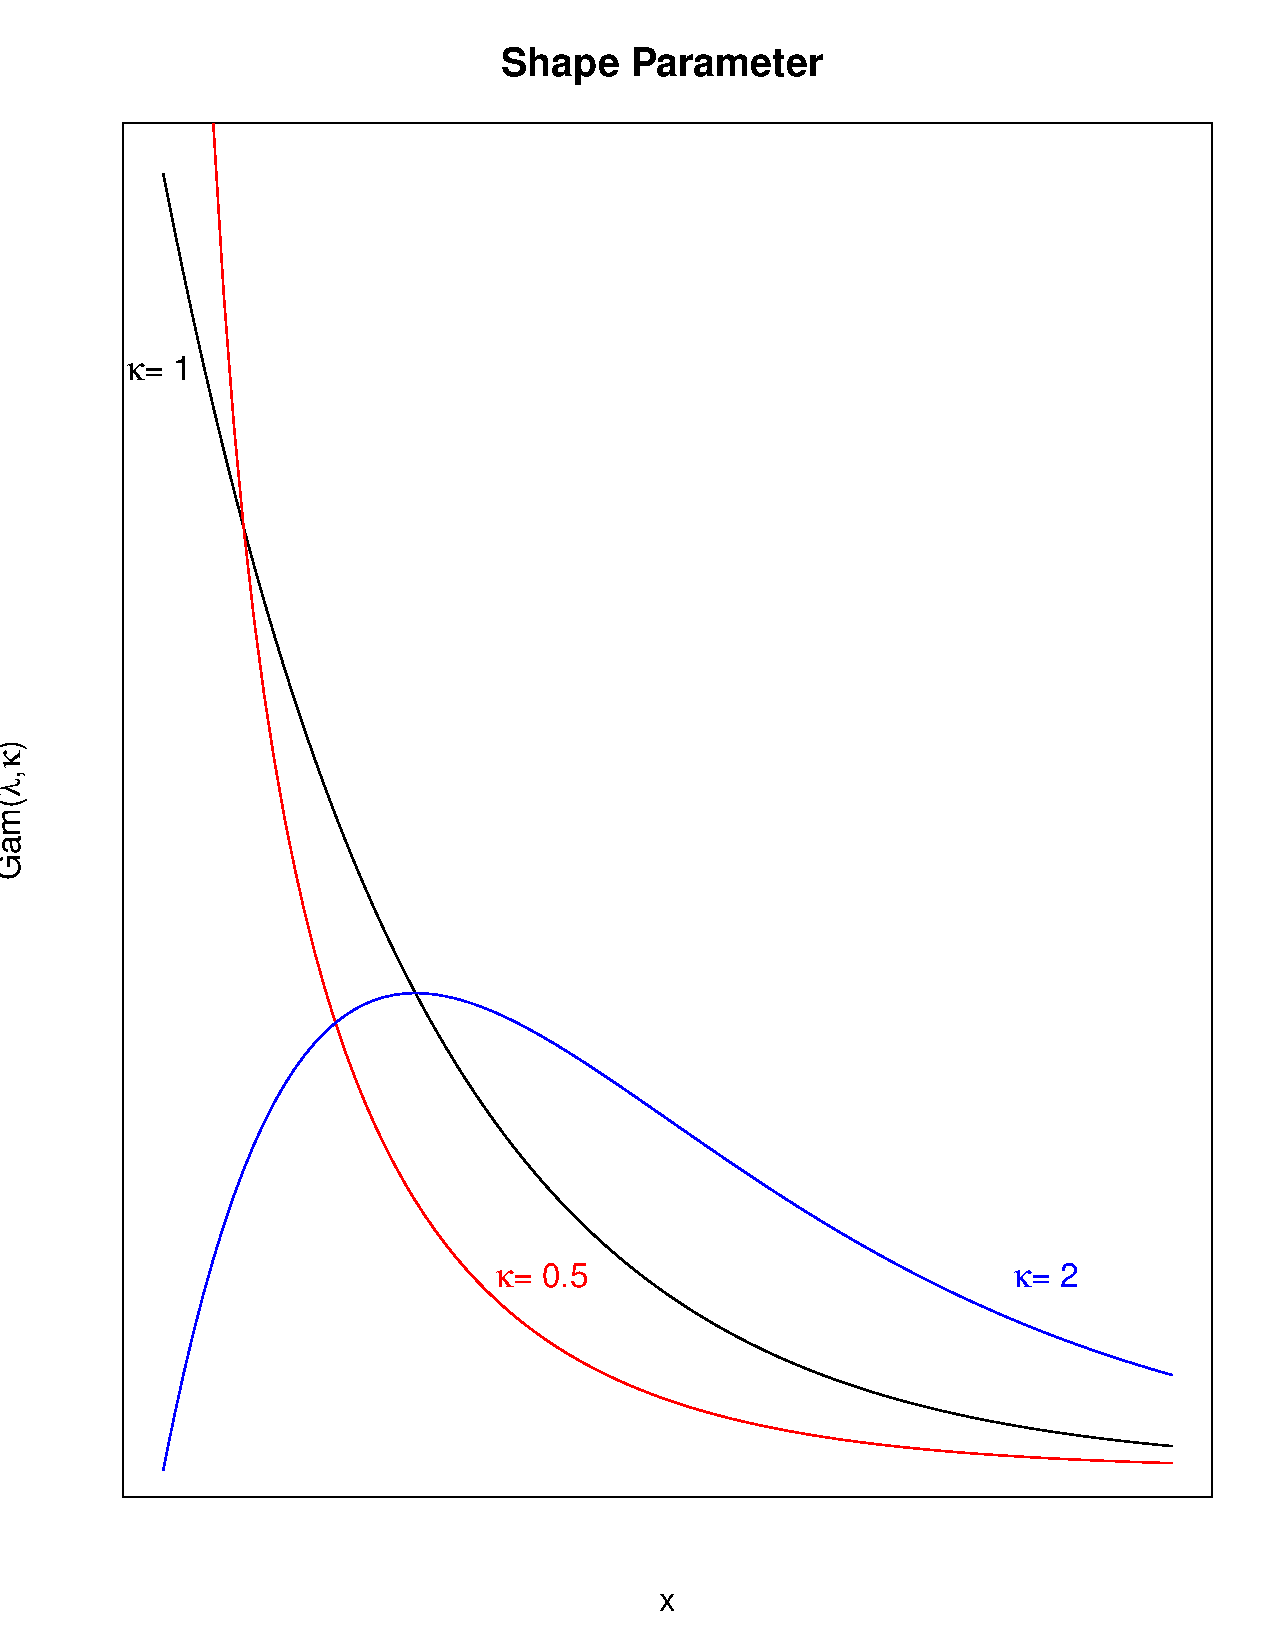
\includegraphics[height=2.5in,width=2.5in]{shape.pdf}

Note that $\lambda$ is a scale parameter.\\\\
Unless $\kappa$ is an integer, we cannot integrate the pdf of the gamma distribution in a closed form, but for integer values of $\kappa$, we have:
$$F(x,\lambda,n) = 1-\sum_{i=0}^n-1 \frac{\left(\lambda x\right)^i}{i!} e^{-\lambda x}$$
As you might guess, this is computed via iterated integration by parts. We will not perform the calculation. Let's move on to expectation and variance.
\subsubsection{Expectation and Variance of the Gamma Distribution}
Let $X \sim Gam(\lambda,\kappa)$.  We compute the expectation of $X$:
$$E(X) = \int_{-\infty}^{infty}x f(x) dx = \int_0^\infty x \frac{\lambda^\kappa}{\Gamma(\kappa)}x^{\kappa-1} e^{-\lambda x} = \frac{\lambda^\kappa}{\Gamma(\kappa)}\int_0^\infty x^{(\kappa+1)-1} e^{-\lambda x}$$
$$ =  \frac{\lambda^\kappa\Gamma(\kappa+1)}{\lambda^{\kappa+1}\Gamma(\kappa)}\int_0^\infty \frac{\lambda^{\kappa+1}}{\Gamma(\kappa+1)}x^{(\kappa+1)-1} e^{-\lambda x}$$
Now, the integrand is the pdf of a $Gam(\lambda,\kappa+1)$ random variable, integrated over its full support, thus:
$$ =  \frac{\lambda^\kappa\Gamma(\kappa+1)}{\lambda^{\kappa+1}\Gamma(\kappa)}\int_0^\infty \frac{\lambda^{\kappa+1}}{\Gamma(\kappa+1)}x^{(\kappa+1)-1} e^{-\lambda x} = \frac{\lambda^\kappa\Gamma(\kappa+1)}{\lambda^{\kappa+1}\Gamma(\kappa)} = \frac{\kappa}{\lambda}$$

where we have used the fact that $\Gamma(\kappa+1) = \kappa\Gamma(\kappa)$. Similarly, we could compute $E(X^2)$:
$$E(X^2) = \frac{\kappa(\kappa+1)}{\lambda^2}$$
so that 
$$Var(X) = E(X^2)-\left(E(X)\right)^2 =   \frac{\kappa(\kappa+1)}{\lambda^2}\left(\frac{\kappa}{\lambda}\right)^2 = \frac{\kappa}{\lambda^2}$$
\paragraph{Related Distributions}
We have already noted that for $\kappa=1$, $Gamm(\lambda,1)=Exp(\lambda)$. There is another special case of the gamma distribution that will come up (a lot!).
$$Gam(2,\frac{\nu}2) =\chi^2_\nu$$
In other words, for $\lambda =2$ and $\kappa=\nu/2$, the gamma distribution is a chi-squared distribution on $\nu$ degrees of freedom.\\\\
This completes our introductory discussion of some named continuous distributions. We will continue to study these distributions as we introduce other topics in probability theory.

\end{document}